\documentclass[aspectratio=169,11pt]{beamer}

% ---------- Pacchetti ----------
\usepackage[utf8]{inputenc}
\usepackage[T1]{fontenc}
\usepackage[italian,provide=*]{babel}
\usepackage{tikz}
\usetikzlibrary{arrows.meta, positioning, shapes.geometric}

% ---------- Colori (tema Second Brain) ----------
\definecolor{sbnavy}{HTML}{1D3557}   % blu notte
\definecolor{sbteal}{HTML}{0E7C86}   % teal/ciano scuro
\definecolor{sbaccent}{HTML}{2A9D8F} % accento
\definecolor{sbgray}{HTML}{6B7280}   % grigio testo secondario
\definecolor{sblight}{HTML}{EAF2F4}  % sfondo chiaro blocchi

% ---------- Tema ----------
\usetheme{default}
\usefonttheme{professionalfonts}
\setbeamertemplate{navigation symbols}{}
\setbeamercolor{frametitle}{fg=sbnavy}
\setbeamercolor{title}{fg=sbnavy}
\setbeamercolor{itemize item}{fg=sbteal}
\setbeamercolor{itemize subitem}{fg=sbaccent}
\setbeamercolor{structure}{fg=sbteal}
\setbeamertemplate{itemize item}{\textbullet}
\setbeamertemplate{itemize subitem}{\textendash}

% blocchi: alternativa (neutro) e scelta (evidenziato)
\setbeamercolor{block title}{bg=sbnavy,fg=white}
\setbeamercolor{block body}{bg=sblight,fg=black}
\setbeamercolor{block title alerted}{bg=sbteal,fg=white}
\setbeamercolor{block body alerted}{bg=sblight,fg=black}

% ---------- Header / Footer (stile Skarab) ----------
\setbeamertemplate{headline}{%
  \ifnum\thepage>1
  \vspace{4pt}%
  \hspace{14pt}\raisebox{-1pt}{\IfFileExists{logo_gruppo_senza_background.png}{
\includegraphics[height=4mm]{logo_gruppo_senza_background.png}}{\scriptsize\color{sbgray}the bitless}}\hfill{\scriptsize\color{sbgray}\insertframenumber/\inserttotalframenumber}\hspace{14pt}%
  \vspace{2pt}%
  \hspace{14pt}{\color{sbnavy}\rule{\dimexpr\paperwidth-28pt\relax}{0.6pt}}%
  \fi
}
\setbeamertemplate{frametitle}{%
  \vspace{2pt}\hspace{2pt}{\large\bfseries\insertframetitle}\par
}
\setbeamertemplate{footline}{%
  \ifnum\thepage>1
  \hspace{14pt}{\color{sbnavy}\rule{\dimexpr\paperwidth-28pt\relax}{0.6pt}}\par
  \vspace{2pt}%
  \hspace{14pt}{\scriptsize\color{sbgray}RTB -- Tecnologie \& PoC}\hfill{\scriptsize\color{sbgray}[INSERIRE DATA]}\hspace{14pt}%
  \vspace{4pt}%
  \fi
}

% comando rapido per blocco "scelto"
\newenvironment{scelto}[1]{\begin{alertblock}{#1}}{\end{alertblock}}

% ---------- Metadati ----------
\title{Tecnologie \& Proof of Concept}
\subtitle{Capitolato C6 --- Second Brain}
\date{[INSERIRE DATA]}

\begin{document}

% ============ SLIDE 1 — COPERTINA ============
{
\setbeamertemplate{headline}{}
\setbeamertemplate{footline}{}
\begin{frame}[plain]
  \vfill
  \begin{center}
    \IfFileExists{logo_gruppo_senza_background.png}{
\includegraphics[height=15mm]{logo_gruppo_senza_background.png}}\\
    {\color{sbnavy}\rule{0.55\textwidth}{1.2pt}}\\[10pt]
    {\Huge\bfseries\color{sbnavy} Tecnologie \& Proof of Concept$_G$}\\[8pt]
    {\large\color{sbteal} Capitolato$_G$ C6 --- Second Brain}\\[4pt]
    {\normalsize\color{sbgray} The Bitless \quad\textbullet\quad Gruppo 18 \quad\textbullet\quad A.A. 2025/2026}\\[6pt]
    {\small\color{sbgray} [INSERIRE DATA]}\\[14pt]
    {\color{sbnavy}\rule{0.55\textwidth}{1.2pt}}\\[12pt]
    {\footnotesize Università degli Studi di Padova --- Ingegneria del Software}\\[6pt]
  \end{center}
  \vfill
\end{frame}
}

% ============ SLIDE 2 — CAPITOLATO$_G$ ============
\begin{frame}{Second Brain}
  \begin{block}{Visione}
    Un editor \textbf{Markdown} affiancato a un \textbf{LLM}: un secondo cervello per scrivere, migliorare e fare brainstorming$_G$.
  \end{block}
  \vspace{2pt}
  \begin{columns}[T]
    \column{0.54\textwidth}
    {\bfseries\small Requisiti$_G$ obbligatori}
    \begin{itemize}
      \item[\textcolor{sbteal}{\textbullet}] {\small Editor Markdown + rendering live}
      \item[\textcolor{sbteal}{\textbullet}] {\small Accesso a un LLM$_G$ sul testo}
      \item[\textcolor{sbteal}{\textbullet}] {\small Riassunto, riscrittura, traduzione}
      \item[\textcolor{sbteal}{\textbullet}] {\small Critica ``Sei cappelli'' di De Bono}
      \item[\textcolor{sbteal}{\textbullet}] {\small Distant Writing$_G$ (testo da prompt)}
      \item[\textcolor{sbteal}{\textbullet}] {\small Salvataggio e lettura note}
    \end{itemize}
    \column{0.46\textwidth}
    \centering
    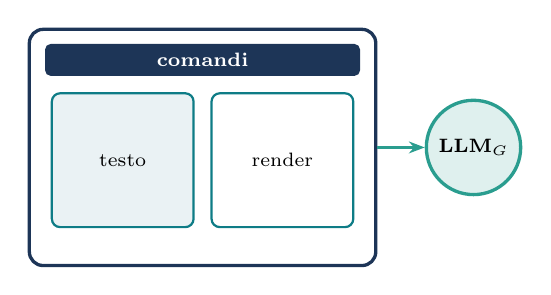
\begin{tikzpicture}[font=\scriptsize]
      % cornice app
      \node[draw=sbnavy, very thick, rounded corners=5pt, minimum width=44mm, minimum height=30mm] (app) {};
      % barra comandi
      \node[fill=sbnavy, text=white, rounded corners=2pt, minimum width=40mm, anchor=north, font=\scriptsize\bfseries] (bar) at ([yshift=-2mm]app.north) {comandi};
      % pannello testo
      \node[draw=sbteal, thick, fill=sblight, rounded corners=3pt, minimum width=18mm, minimum height=17mm, below left=2mm and 1mm of bar.south, anchor=north east] (txt) {testo};
      % pannello render
      \node[draw=sbteal, thick, fill=white, rounded corners=3pt, minimum width=18mm, minimum height=17mm, below right=2mm and 1mm of bar.south, anchor=north west] (rnd) {render};
      % LLM$_G$
      \node[draw=sbaccent, very thick, fill=sbaccent!15, circle, minimum size=11mm, right=6mm of app, font=\scriptsize\bfseries] (llm$_G$) {LLM$_G$};
      \draw[-{Stealth[length=2mm]}, very thick, sbaccent] (app.east) -- (llm$_G$.west);
    \end{tikzpicture}\\[2pt]
    {\scriptsize\color{sbgray} editor a 2 pannelli + accesso LLM$_G$}
  \end{columns}
  \vspace{2pt}
\end{frame}

% ============ SLIDE 3 — ARCHITETTURA (TikZ) ============
\begin{frame}{Architettura}
  \vspace{6pt}
  \begin{center}
  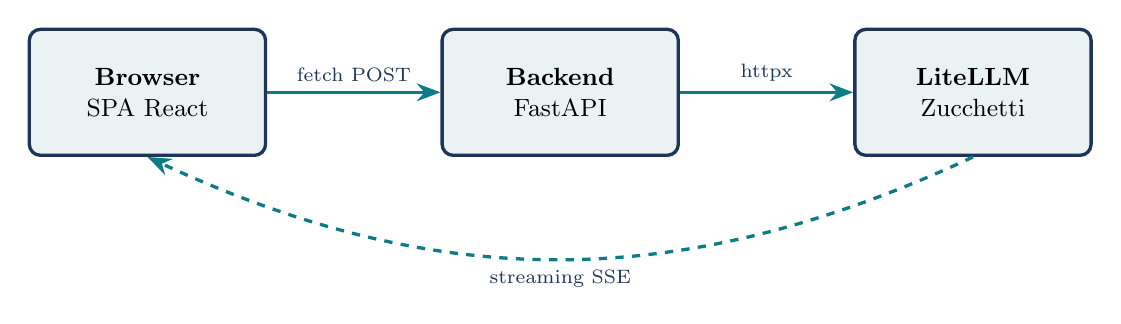
\begin{tikzpicture}[
    node distance=22mm,
    box/.style={rectangle, rounded corners=4pt, draw=sbnavy, very thick,
                fill=sblight, minimum width=30mm, minimum height=16mm,
                align=center, font=\small},
    arr/.style={-{Stealth[length=3mm]}, very thick, draw=sbteal}
  ]
    \node[box] (web) {\textbf{Browser}\\ SPA React};
    \node[box, right=of web] (api$_G$) {\textbf{Backend}\\ FastAPI};
    \node[box, right=of api$_G$] (llm$_G$) {\textbf{LiteLLM}\\ Zucchetti};
    \draw[arr] (web) -- node[above, font=\scriptsize, text=sbnavy] {fetch POST} (api$_G$);
    \draw[arr] (api$_G$) -- node[above, font=\scriptsize, text=sbnavy] {httpx} (llm$_G$);
    \draw[arr, dashed] (llm$_G$.south) to[bend left=25] node[below, font=\scriptsize, text=sbnavy] {streaming SSE} (web.south);
  \end{tikzpicture}
  \end{center}
  \vspace{4pt}
  \begin{itemize}
    \item Streaming \textbf{end-to-end} con effetto macchina da scrivere
    \item Backend \textbf{stateless}: nessuna logica di dominio$_G$ lato server
  \end{itemize}
\end{frame}

% ============ SLIDE 4 — FRONTEND$_G$ ============
\begin{frame}{Tecnologie --- Frontend$_G$}
  \begin{itemize}
    \item \textbf{React 19 + TypeScript + Vite} --- ecosistema maturo, tipi statici, dev server rapido
    \item \textbf{CodeMirror 6} --- editor Markdown leggero (\textasciitilde100\,KB), undo/redo e highlighting nativi
    \item \textbf{react-markdown + plugin} --- pipeline Markdown$\to$AST, anti-XSS, tabelle e LaTeX$_G$
    \item \textbf{Zustand} --- stato globale senza boilerplate, re-render minimi
    \item \textbf{Tailwind v4 + shadcn/ui} --- componenti modificabili, no lock-in, tema chiaro/scuro
  \end{itemize}
  \vspace{2pt}
  \begin{center}
  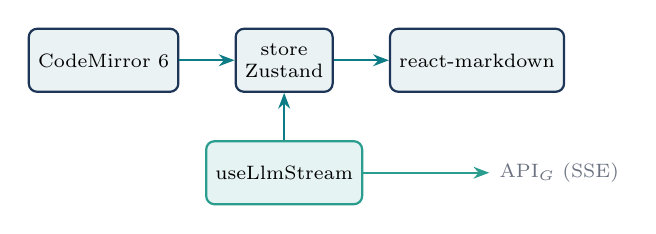
\begin{tikzpicture}[font=\scriptsize, node distance=7mm,
     comp/.style={draw=sbnavy, thick, rounded corners=3pt, fill=sblight, minimum height=8mm, align=center},
     a/.style={-{Stealth[length=2mm]}, thick, sbteal}]
    \node[comp] (cm) {CodeMirror 6};
    \node[comp, right=of cm] (st) {store\\Zustand};
    \node[comp, right=of st] (md) {react-markdown};
    \node[comp, draw=sbaccent, fill=sbaccent!12, below=6mm of st] (hk) {useLlmStream};
    \draw[a] (cm) -- (st);
    \draw[a] (st) -- (md);
    \draw[a] (hk) -- (st);
    \draw[a, sbaccent] (hk.east) -- ++(1.6,0) node[right, text=sbgray] {API$_G$ (SSE)};
  \end{tikzpicture}
  \end{center}
\end{frame}

% ============ SLIDE 5 — CONFRONTO EDITOR ============
\begin{frame}{Editor --- CodeMirror 6 vs alternative}
  \begin{columns}[T]
    \column{0.33\textwidth}
    \begin{block}{textarea HTML}
      {\small Semplice, ma niente highlighting Markdown né undo/redo strutturato. Accessibilità da costruire.}
    \end{block}
    \column{0.33\textwidth}
    \begin{block}{Monaco (VS Code)}
      {\small Potentissimo ma pesante (vari MB), pensato per l'IDE: eccessivo per Markdown.}
    \end{block}
    \column{0.33\textwidth}
    \begin{scelto}{CodeMirror 6 \ensuremath{\checkmark}}
      {\small Leggero e modulare: highlighting, undo/redo e accessibilità nativi, API$_G$ tipizzata.}
    \end{scelto}
  \end{columns}
  \vspace{6pt}
  \begin{center}
    {\color{sbnavy}\small Il giusto compromesso tra potenza e leggerezza per il nostro caso d'uso.}
  \end{center}
\end{frame}

% ============ SLIDE 6 — BACKEND ============
\begin{frame}{Tecnologie --- Backend}
  \begin{itemize}
    \item \textbf{Python 3.12 + FastAPI} --- async nativo per lo streaming LLM$_G$, OpenAPI autogenerato
    \item \textbf{Pydantic v2} --- validazione$_G$ runtime, errori 422 espliciti, base per i tipi TypeScript
    \item \textbf{httpx async} --- streaming nativo e propagazione dell'annullamento fino al provider
    \item \textbf{Astrazione ``LLMClient''} --- interfaccia astratta sopra il provider, per testabilità ed estensioni
  \end{itemize}
\end{frame}

% ============ SLIDE 7 — CONFRONTO BACKEND ============
\begin{frame}{Backend --- FastAPI vs Node.js/Express}
  \begin{columns}[T]
    \column{0.5\textwidth}
    \begin{block}{Node.js + Express}
      {\small Ecosistema JS unico FE+BE, ma lo streaming LLM$_G$ richiede gestire a mano async e backpressure; validazione$_G$ e OpenAPI da aggiungere con librerie esterne.}
    \end{block}
    \column{0.5\textwidth}
    \begin{scelto}{FastAPI \ensuremath{\checkmark}}
      {\small Async nativo per stream lunghi senza bloccare; validazione$_G$ Pydantic e OpenAPI integrate; dall'OpenAPI generiamo i tipi TypeScript del frontend$_G$.}
    \end{scelto}
  \end{columns}
  \vspace{6pt}
  \begin{center}
    {\color{sbnavy}\small Il cuore del progetto è lo streaming LLM$_G$: FastAPI lo gestisce nativamente.}
  \end{center}
\end{frame}

% ============ SLIDE 8 — CONFRONTO ACCESSO LLM$_G$ ============
\begin{frame}{Accesso all'LLM$_G$ --- astrazione vs chiamata diretta}
  \begin{columns}[T]
    \column{0.5\textwidth}
    \begin{block}{Chiamata diretta al provider}
      {\small Meno codice subito, ma le route restano accoppiate al provider concreto: cambiarlo o aggiungerne uno impone di riscriverle, e i test$_G$ richiedono l'LLM$_G$ reale.}
    \end{block}
    \column{0.5\textwidth}
    \begin{scelto}{LLMClient astratto + LiteLLMClient \ensuremath{\checkmark}}
      {\small Le route dipendono dall'interfaccia, non dal provider: cambiarlo = modifica di config; testabile con mock pytest senza chiamare l'LLM$_G$.}
    \end{scelto}
  \end{columns}
  \vspace{6pt}
  {\small\color{sbgray} Oggi provider unico (LiteLLM Zucchetti); l'astrazione tiene aperta la porta a estensioni future.}
\end{frame}

% ============ SLIDE 9 — INFRA & QUALITÀ ============
\begin{frame}{Infrastruttura \& Qualità}
  \begin{columns}[T]
    \column{0.5\textwidth}
    {\bfseries Infrastruttura}
    \begin{itemize}
      \item Docker Compose --- ambiente riproducibile in un comando
      \item Mono-repo --- frontend$_G$ + backend, CI unificata
    \end{itemize}
    \column{0.5\textwidth}
    {\bfseries Qualità}
    \begin{itemize}
      \item GitHub$_G$ Actions --- CI: lint, type check, test$_G$, build
      \item Test$_G$: Vitest + Playwright (FE), pytest (BE)
      \item openapi-typescript --- tipi TS dal backend, zero disallineamenti
    \end{itemize}
  \end{columns}
\end{frame}

% ============ SLIDE 10 — POC$_G$ OBIETTIVO ============
\begin{frame}{Proof of Concept$_G$ --- obiettivo}
  \begin{block}{Obiettivo}
    Validare la pipeline di \textbf{streaming LLM end-to-end} con una sola funzione: il \textbf{riassunto}.
  \end{block}
  \vspace{4pt}
  \begin{center}
  
\begin{tikzpicture}[
    flowstep/.style={rectangle, rounded corners=3pt, draw=sbteal, thick, fill=sblight,
                 align=center, font=\scriptsize, minimum height=10mm, text width=24mm},
    arr/.style={-{Stealth[length=2.5mm]}, thick, draw=sbnavy}
  ]
    \node[flowstep] (a) {Utente scrive\\ in Markdown};
    \node[flowstep, right=10mm of a] (b) {Click\\ ``Genera Riassunto''};
    \node[flowstep, right=10mm of b] (c) {Output$_G$ in\\ streaming};
    \draw[arr] (a) -- (b);
    \draw[arr] (b) -- (c);
  \end{tikzpicture}
  \end{center}
  \vspace{2pt}
  {\color{sbnavy}\small Le altre funzioni AI (traduzione, riscrittura, Sei Cappelli, Distant Writing$_G$) differiscono \textbf{solo per il prompt}: l'architettura resta identica.}
\end{frame}

% ============ SLIDE 11 — POC$_G$ VALIDAZIONE$_G$ ============
\begin{frame}{Proof of Concept$_G$ --- cosa abbiamo validato}
  \begin{itemize}
    \item[\textcolor{sbaccent}{\ensuremath{\checkmark}}] Streaming fluido (effetto macchina da scrivere), UI mai bloccata
    \item[\textcolor{sbaccent}{\ensuremath{\checkmark}}] Interruzione propagata su tutta la catena (client $\to$ server $\to$ provider)
    \item[\textcolor{sbaccent}{\ensuremath{\checkmark}}] Errori del provider gestiti con messaggio chiaro, testo dell'editor preservato
    \item[\textcolor{sbaccent}{\ensuremath{\checkmark}}] Chiave API$_G$ mai esposta al client
    \item[\textcolor{sbaccent}{\ensuremath{\checkmark}}] Ambiente riproducibile da zero con \texttt{docker compose up}
  \end{itemize}
\end{frame}

% ============ SLIDE 12 — CONCLUSIONI ============
\begin{frame}{Contatti}
  \begin{center}
    {\Large\bfseries\color{sbnavy} The Bitless}\\[4pt]
    {\color{sbgray} thebitlessgroup.swe@gmail.com \\ \url{https://thebitless.live/}}
  \end{center}
\end{frame}

\end{document}